\PassOptionsToPackage{unicode=true}{hyperref} % options for packages loaded elsewhere
\PassOptionsToPackage{hyphens}{url}
%
\documentclass[]{book}
\usepackage{lmodern}
\usepackage{amssymb,amsmath}
\usepackage{ifxetex,ifluatex}
\usepackage{fixltx2e} % provides \textsubscript
\ifnum 0\ifxetex 1\fi\ifluatex 1\fi=0 % if pdftex
  \usepackage[T1]{fontenc}
  \usepackage[utf8]{inputenc}
  \usepackage{textcomp} % provides euro and other symbols
\else % if luatex or xelatex
  \usepackage{unicode-math}
  \defaultfontfeatures{Ligatures=TeX,Scale=MatchLowercase}
\fi
% use upquote if available, for straight quotes in verbatim environments
\IfFileExists{upquote.sty}{\usepackage{upquote}}{}
% use microtype if available
\IfFileExists{microtype.sty}{%
\usepackage[]{microtype}
\UseMicrotypeSet[protrusion]{basicmath} % disable protrusion for tt fonts
}{}
\IfFileExists{parskip.sty}{%
\usepackage{parskip}
}{% else
\setlength{\parindent}{0pt}
\setlength{\parskip}{6pt plus 2pt minus 1pt}
}
\usepackage{hyperref}
\hypersetup{
            pdftitle={Doing Democratic Data Analysis},
            pdfauthor={Corban Nemeth},
            pdfborder={0 0 0},
            breaklinks=true}
\urlstyle{same}  % don't use monospace font for urls
\usepackage{color}
\usepackage{fancyvrb}
\newcommand{\VerbBar}{|}
\newcommand{\VERB}{\Verb[commandchars=\\\{\}]}
\DefineVerbatimEnvironment{Highlighting}{Verbatim}{commandchars=\\\{\}}
% Add ',fontsize=\small' for more characters per line
\usepackage{framed}
\definecolor{shadecolor}{RGB}{248,248,248}
\newenvironment{Shaded}{\begin{snugshade}}{\end{snugshade}}
\newcommand{\AlertTok}[1]{\textcolor[rgb]{0.94,0.16,0.16}{#1}}
\newcommand{\AnnotationTok}[1]{\textcolor[rgb]{0.56,0.35,0.01}{\textbf{\textit{#1}}}}
\newcommand{\AttributeTok}[1]{\textcolor[rgb]{0.77,0.63,0.00}{#1}}
\newcommand{\BaseNTok}[1]{\textcolor[rgb]{0.00,0.00,0.81}{#1}}
\newcommand{\BuiltInTok}[1]{#1}
\newcommand{\CharTok}[1]{\textcolor[rgb]{0.31,0.60,0.02}{#1}}
\newcommand{\CommentTok}[1]{\textcolor[rgb]{0.56,0.35,0.01}{\textit{#1}}}
\newcommand{\CommentVarTok}[1]{\textcolor[rgb]{0.56,0.35,0.01}{\textbf{\textit{#1}}}}
\newcommand{\ConstantTok}[1]{\textcolor[rgb]{0.00,0.00,0.00}{#1}}
\newcommand{\ControlFlowTok}[1]{\textcolor[rgb]{0.13,0.29,0.53}{\textbf{#1}}}
\newcommand{\DataTypeTok}[1]{\textcolor[rgb]{0.13,0.29,0.53}{#1}}
\newcommand{\DecValTok}[1]{\textcolor[rgb]{0.00,0.00,0.81}{#1}}
\newcommand{\DocumentationTok}[1]{\textcolor[rgb]{0.56,0.35,0.01}{\textbf{\textit{#1}}}}
\newcommand{\ErrorTok}[1]{\textcolor[rgb]{0.64,0.00,0.00}{\textbf{#1}}}
\newcommand{\ExtensionTok}[1]{#1}
\newcommand{\FloatTok}[1]{\textcolor[rgb]{0.00,0.00,0.81}{#1}}
\newcommand{\FunctionTok}[1]{\textcolor[rgb]{0.00,0.00,0.00}{#1}}
\newcommand{\ImportTok}[1]{#1}
\newcommand{\InformationTok}[1]{\textcolor[rgb]{0.56,0.35,0.01}{\textbf{\textit{#1}}}}
\newcommand{\KeywordTok}[1]{\textcolor[rgb]{0.13,0.29,0.53}{\textbf{#1}}}
\newcommand{\NormalTok}[1]{#1}
\newcommand{\OperatorTok}[1]{\textcolor[rgb]{0.81,0.36,0.00}{\textbf{#1}}}
\newcommand{\OtherTok}[1]{\textcolor[rgb]{0.56,0.35,0.01}{#1}}
\newcommand{\PreprocessorTok}[1]{\textcolor[rgb]{0.56,0.35,0.01}{\textit{#1}}}
\newcommand{\RegionMarkerTok}[1]{#1}
\newcommand{\SpecialCharTok}[1]{\textcolor[rgb]{0.00,0.00,0.00}{#1}}
\newcommand{\SpecialStringTok}[1]{\textcolor[rgb]{0.31,0.60,0.02}{#1}}
\newcommand{\StringTok}[1]{\textcolor[rgb]{0.31,0.60,0.02}{#1}}
\newcommand{\VariableTok}[1]{\textcolor[rgb]{0.00,0.00,0.00}{#1}}
\newcommand{\VerbatimStringTok}[1]{\textcolor[rgb]{0.31,0.60,0.02}{#1}}
\newcommand{\WarningTok}[1]{\textcolor[rgb]{0.56,0.35,0.01}{\textbf{\textit{#1}}}}
\usepackage{longtable,booktabs}
% Fix footnotes in tables (requires footnote package)
\IfFileExists{footnote.sty}{\usepackage{footnote}\makesavenoteenv{longtable}}{}
\usepackage{graphicx,grffile}
\makeatletter
\def\maxwidth{\ifdim\Gin@nat@width>\linewidth\linewidth\else\Gin@nat@width\fi}
\def\maxheight{\ifdim\Gin@nat@height>\textheight\textheight\else\Gin@nat@height\fi}
\makeatother
% Scale images if necessary, so that they will not overflow the page
% margins by default, and it is still possible to overwrite the defaults
% using explicit options in \includegraphics[width, height, ...]{}
\setkeys{Gin}{width=\maxwidth,height=\maxheight,keepaspectratio}
\setlength{\emergencystretch}{3em}  % prevent overfull lines
\providecommand{\tightlist}{%
  \setlength{\itemsep}{0pt}\setlength{\parskip}{0pt}}
\setcounter{secnumdepth}{5}
% Redefines (sub)paragraphs to behave more like sections
\ifx\paragraph\undefined\else
\let\oldparagraph\paragraph
\renewcommand{\paragraph}[1]{\oldparagraph{#1}\mbox{}}
\fi
\ifx\subparagraph\undefined\else
\let\oldsubparagraph\subparagraph
\renewcommand{\subparagraph}[1]{\oldsubparagraph{#1}\mbox{}}
\fi

% set default figure placement to htbp
\makeatletter
\def\fps@figure{htbp}
\makeatother

\usepackage{booktabs}
\usepackage[]{natbib}
\bibliographystyle{apalike}

\title{Doing Democratic Data Analysis}
\author{Corban Nemeth}
\date{2020-05-06}

\begin{document}
\maketitle

{
\setcounter{tocdepth}{1}
\tableofcontents
}
\hypertarget{preface}{%
\chapter*{Preface}\label{preface}}
\addcontentsline{toc}{chapter}{Preface}

I believe that data, \emph{in the hands of public administrators and policy analysts}\footnote{\emph{Not IT departments}}, has the power to transform the way government works.

Big questions will, and should, be asked of big data--- the role of government in regulating algorithmic bias, facial recognition, and consumer data privacy is a vital conversation. However, these topics should not detract or deter public administrators and policy analysts from leaning into \textbf{small data} for decision-making purposes.

Public administrators and analysts who are data literate will be able to make and inform better decisions while avoiding the pitfalls posed by the latest technological trends. This book represents an opportunity for public administrators and policy analysts to join their subject matter expertise with foundation principles and practices of democratic data analysis--- data analysis that is \textbf{transparent, relevant, and grounded in the context of ethical and effective governance}.

In this guide, I present an opinionated framework for data analysis in public sector organizations. By opinionated, I mean that I will teach you what I think is the right way to do things given my own experience as a public sector policy and data analyst. Your experience might differ-- and that's great. I hope that where you can use your experience in place of mine, you do to the fullest extent. With that in mind, it is often said that you have to know the rules to break them, so I will teach you the ``rules'' as I understand them.

This is guide is not an excel how-to manual. My hope is that the principles and practices outlined here will allow you to explore whatever analysis tools you are interested in in a democratic manner. With that said, practical examples are given in Excel and in R.

\hypertarget{intro}{%
\chapter{Introduction}\label{intro}}

\begin{quote}
Data analysis is a process of inspecting, cleansing, transforming, and modeling data with the goal of discovering useful information, informing conclusions and supporting decision-making.
\end{quote}

-*Wikipedia (shame on me)

\hypertarget{principles-and-practices}{%
\section{Principles and Practices}\label{principles-and-practices}}

In this handbook, I propose four principles of democratic data analysis. Democratic data analysis is:
* Tidy
* Reproducible,
* Uncertainty-oriented, and
* Audience-focused

As this isn't a how-to manual, each chapter will begin with a description of the \emph{principles} outlined above and arguments for why they are important. This will be followed by \emph{practices} section where I walk through examples of how to implement these principles in common situations and provide additional materials for you to learn how to apply these principles using common data analysis tools.

Why maintain the distinction between principles and practices? Data analysis is driven by the technologies that we have access to. Whether it be the venerable pivot table, or a new-school dashboard platform, or a data-oriented programming language, the principles that I lay out in this handbook supersede specific technologies. Think of it like grammar. You may write by hand, on a computer, using text-to-speech. You may be writing a poem, a novel, an argument, or an instruction manual. But the basic rules of grammar are relevant in whatever medium you choose. Similarly, this guide will teach you the basic ``grammar'' of democratic data analysis. This will allow you to apply this knowledge in whatever platform or technology you are interested in or have access to. But similar to learning language, it helps to practice. It isn't much to use to study grammar without ever writing a sentance.

The principles section of this guide will include examples in both Excel and \texttt{R}. Government runs on Excel, so all of the examples and exercises will be Excel compatible. If you are comfortable with Excel\footnote{aka you use \texttt{vlookup}, \texttt{index(match)}, pivot tables, or \emph{Get \& Transform} on a somewhat regular basis} and want to challenge yourself, boost your resume, and become a data superstar, I would highly recommend learning \texttt{R}.

\hypertarget{what-is-data-analysis}{%
\section{What is data analysis?}\label{what-is-data-analysis}}

Data analysis is the process of transforming numbers on a page to insight into the real world. It's looking at a table and gaining insight from it. Data analysis can be as simple as adding totals into a column to see cumulative effects, or as complicated as time-series forecasting. But fundamentally, all data analysis is taking inputs and applying those inputs to the real world to gain insight into the real world. It also may be helpful to think about what data analysis \emph{isn't}:

\begin{enumerate}
\def\labelenumi{\arabic{enumi}.}
\tightlist
\item
  Data analysis isn't math.
\end{enumerate}

\begin{itemize}
\tightlist
\item
  Calculations are great, but \texttt{a7\ +\ b8} in Excel is deterministic. It gives you one answer. This book is not interested in data analysis that gives you the right answer, because there is no such thing. There are many answers to many questions, depending on how those questions are asked and how the data is analyzed.
\end{itemize}

\begin{enumerate}
\def\labelenumi{\arabic{enumi}.}
\setcounter{enumi}{1}
\tightlist
\item
  Data analysis isn't statistics.
\end{enumerate}

\begin{itemize}
\tightlist
\item
  This book is about reading and telling the story of your data in a way that can complement expertise and experience to make better decisions. Statistics are often used as a cheap stand-in for domain expertise and are often abused in favor of trusting the analyst or administrator to back up their assumptions with both quantitative and qualitative data.
\end{itemize}

\begin{enumerate}
\def\labelenumi{\arabic{enumi}.}
\setcounter{enumi}{2}
\tightlist
\item
  Data analysis isn't research methods.
\end{enumerate}

\begin{itemize}
\tightlist
\item
  No set of tools and practices can stand in for asking the right questions, and transforming data into information to answer that question. This book will give you the tools to work with your quantitative data to answer relevant questions, but all good analysis begins with a good question.
\end{itemize}

\hypertarget{the-grammar-of-data-analysis}{%
\section[The Grammar of Data Analysis]{\texorpdfstring{The Grammar of Data Analysis\footnote{Adapted from Hadley Wickham's paper on \href{https://vita.had.co.nz/papers/tidy-data.pdf}{Tidy Data}}}{The Grammar of Data Analysis}}\label{the-grammar-of-data-analysis}}

As I mentioned before, democratic data analysis has an underlying structure, like a sentance There are rules so these sentences (hopefully) make sense to you, the reader. Similarly, by following common conventions of democratic data analysis, others will be able to ``read'' your analysis like you are reading this sentence. And also, like grammar, you can break the rules-- but it helps to know them first.

Here are a couple definitions that will help as you move through this text. Don't worry about memorizing them, as I will refer back to these definitions frequently.

\begin{itemize}
\tightlist
\item
  Fields

  \begin{itemize}
  \tightlist
  \item
    A field is a fancy name for a column. From here on out, every calculation, manipulation, formula, you name it, will be on a column. I want you to forget that you could ever modify a lone cell in Excel. No more formulas in cells. No more typing in values to a cell. Certainly no more writing over data in a cell. Democratic data analysis depends on formulas that work on entire fields. Everything you would need to do to a single cell in Excel can-- and should!-- be done to an entire column.
  \end{itemize}
\item
  Variables

  \begin{itemize}
  \tightlist
  \item
    A variable is something in your data that can change. That's it! Variables become very important when looking at how to structure your data. Each variable should have its own field.
  \end{itemize}
\item
  Observations

  \begin{itemize}
  \tightlist
  \item
    Observations make up the rows of your data set. Each observation should correspond to a specific ``thing.'' This will make more sense later, I promise.
  \end{itemize}
\item
  Values

  \begin{itemize}
  \tightlist
  \item
    Values are the actual data in your table. Each value belongs to 1 (one) observation and 1 (one) variable.
  \end{itemize}
\item
  Table

  \begin{itemize}
  \tightlist
  \item
    A table is the grouping of all observations of a similar type.
  \end{itemize}
\end{itemize}

You may already be able to see how these definitions foreshadow some of what is coming in later sections. For example, there are no references to cells. This is intentional. The most important distinction between democratic data analysis and simply working in excel is that in democratic data analysis, (virtually) \emph{everything} is done on the \texttt{field} level. Changes are made to entire columns, calculations are made on entire columns. Thinking in \texttt{fields} is the first step on the path to democratic data enlightenment. Having data formatted in the structure outlined above forces good data hygiene that will pay massive dividends later on.

\hypertarget{tidy-data}{%
\chapter{Tidy Data}\label{tidy-data}}

Tidy data refers to having your data organized in a specific manner suitable for analysis. An obscene amount of time in data analysis is spent getting data into a tidy format. This chapter will walk through common problems and approaches in cleaning and tidying your data, that will make it easier for others to follow and easier for you to work across technologies and subject areas. Keeping your data in a tidy format for analysis will help because it is a fundamentally flexible way of working with data. Keeping scattered, lose data in spreadsheets is a sure way to cause confusion for yourself and others.

\hypertarget{the-importance-of-tables}{%
\section{The Importance of Tables}\label{the-importance-of-tables}}

If I could convince you of one thing, it would be the value in keeping your data in a table-based excel format. Again, this is true for data analysis purposes. If you are trying to do math or statistics, then the table based framework can sometimes fall short. But if you are concerned with working with data to draw conclusions, then tables are the way to go.

\hypertarget{cleaning-vs-tidying}{%
\section{Cleaning vs Tidying}\label{cleaning-vs-tidying}}

I hate cleaning, but love tidying. Unfortunately, as in with life, one must clean before one tidies. But let's start with some conceptual definitions.

Cleaning refers to the process of scrubbing the data into a way that makes sense to you, the analyst. Oftentimes, and especially in public sector organizations, the data is not clean. Whether you are looking at the output of a SurveyMonkey survey or a canned report that is run from the IT department, your data will come in all shapes and sizes. Cleaning data is the process of transforming data values into ones that make sense for the purposes of your analysis.

Here is the first major departure from what you may have been taught about data analysis in Excel. When you get messy data \emph{do not} change individual cell values (if you can at all help it). Recall from the introductory chapter the difference between cells and fields. Fields, as a reminder, are columns that represent one variable. Whenever possible, use data analysis tools to make changes to the entire field, rather than specific cells. Most data analysis software, outside of Excel, make it difficult or impossible to change individual cell values. This is important for several reasons, most of which we will get to in the next chapter on reproducibility. But for now, thinking in terms of fields, and making changes to entire fields, will save you \emph{a lot} of work and headache in the long run. Let's look at a sample dataset that may be similar to one you would encounter in real life. Here is a survey collected by a field manager of a local parks and recreation department on employment.

\begin{Shaded}
\begin{Highlighting}[]
\KeywordTok{library}\NormalTok{(tidyverse)}
\KeywordTok{library}\NormalTok{(DT)}

\NormalTok{sites <-}\StringTok{ }\KeywordTok{tribble}\NormalTok{(}
  \OperatorTok{~}\StringTok{"Employee"}\NormalTok{, }\OperatorTok{~}\StringTok{"Location"}\NormalTok{, }\OperatorTok{~}\StringTok{"Telecommute?"}\NormalTok{, }\OperatorTok{~}\StringTok{"Hire Date"}\NormalTok{,}
  \StringTok{"ron swanson"}\NormalTok{, }\StringTok{"Pawnee City Hall"}\NormalTok{, }\StringTok{"never"}\NormalTok{, }\StringTok{"Unknown"}\NormalTok{,}
  \StringTok{"Knope, Leslie"}\NormalTok{, }\StringTok{"Field Duty"}\NormalTok{, }\StringTok{"1 day/week"}\NormalTok{, }\StringTok{"2011-6-1"}\NormalTok{,}
  \StringTok{"Andy Dwyer"}\NormalTok{, }\StringTok{"sullivan street pit"}\NormalTok{, }\StringTok{"40 hours"}\NormalTok{, }\StringTok{"March 1, 2013"}\NormalTok{,}
  \StringTok{"Jerry Gergich"}\NormalTok{, }\StringTok{"City Hall"}\NormalTok{, }\StringTok{"never"}\NormalTok{, }\StringTok{"6/1/1985"}\NormalTok{,}
  \StringTok{"Garry Gergich"}\NormalTok{, }\StringTok{"City Hall"}\NormalTok{, }\StringTok{"never"}\NormalTok{, }\StringTok{"6/1/1985"}\NormalTok{,}
  \StringTok{"ben wyatt"}\NormalTok{, }\StringTok{"Partridge, Minnesota"}\NormalTok{,}\StringTok{""}\NormalTok{ , }\StringTok{"Jan. 1, 2010"}
\NormalTok{)}

\NormalTok{sites }\OperatorTok\StringTok{ }\KeywordTok{datatable}\NormalTok{(}
    \DataTypeTok{extensions =} \StringTok{'Buttons'}\NormalTok{, }
    \DataTypeTok{options =} \KeywordTok{list}\NormalTok{(}\DataTypeTok{dom =} \StringTok{'Bfrtip'}\NormalTok{, }
                   \DataTypeTok{buttons =} \StringTok{'excel'}\NormalTok{,}
                   \DataTypeTok{searching =} \OtherTok{FALSE}\NormalTok{))}
\end{Highlighting}
\end{Shaded}

\hypertarget{htmlwidget-216e490c2d9a95d0cebe}{}

In this example, it would be trivial to go in to the Excel file and clean up the dates, names, and locations by hand. However, you could imagine this survey replicated for a department of forty employees. It quickly becomes unfeasable to make those edits by hand. When this is the case, there are functions in Excel and R that will make your life much easier.

Here is annotated code for how I would go about cleaning this table in R. The friendly syntax of the \texttt{tidyverse} packages makes it easy to follow along, even if you aren't comfortable writing it yourself. You can accomplish all these similar transformations using \href{https://support.microsoft.com/en-us/office/power-query-101-008b3f46-5b14-4f8b-9a07-d3da689091b5}{Get \& Transform in Excel}.

\begin{Shaded}
\begin{Highlighting}[]
\CommentTok{#creating a new table called "sites_cleaned", starting with the old table "sites"}
\NormalTok{sites_cleaned <-}\StringTok{ }\NormalTok{sites }\OperatorTok\StringTok{ }
\StringTok{  }\CommentTok{#switching the order of names that are backwards}
\StringTok{  }\KeywordTok{mutate}\NormalTok{(}\DataTypeTok{Employee =} \KeywordTok{if_else}\NormalTok{(Employee }\OperatorTok{==}\StringTok{ "Knope, Leslie"}\NormalTok{, }\StringTok{"Leslie Knope"}\NormalTok{, Employee)) }\OperatorTok\StringTok{ }
\StringTok{  }\CommentTok{#seperate employee names into two columns}
\StringTok{  }\KeywordTok{separate}\NormalTok{(Employee, }\DataTypeTok{into =} \KeywordTok{c}\NormalTok{(}\StringTok{"first_name"}\NormalTok{, }\StringTok{"last_name"}\NormalTok{)) }\OperatorTok\StringTok{ }
\StringTok{  }\CommentTok{#renaming column names to standard format}
\StringTok{  }\KeywordTok{rename}\NormalTok{(}\DataTypeTok{location =}\NormalTok{ Location,}
         \DataTypeTok{telecommute_hours =}\StringTok{`}\DataTypeTok{Telecommute?}\StringTok{`}\NormalTok{,}
         \DataTypeTok{hire_date =} \StringTok{`}\DataTypeTok{Hire Date}\StringTok{`}\NormalTok{) }\OperatorTok\StringTok{ }
\StringTok{  }\CommentTok{#changing first and last names and locations to Title Case}
\StringTok{  }\KeywordTok{mutate}\NormalTok{(}\DataTypeTok{first_name =} \KeywordTok{str_to_title}\NormalTok{(first_name),}
         \DataTypeTok{last_name =} \KeywordTok{str_to_title}\NormalTok{(last_name),}
         \DataTypeTok{location =} \KeywordTok{str_to_title}\NormalTok{(location)) }\OperatorTok\StringTok{ }
\StringTok{  }\CommentTok{#coding location data to three categories, In Office, In Field, or Other}
\StringTok{  }\KeywordTok{mutate}\NormalTok{(}\DataTypeTok{location =} \KeywordTok{case_when}\NormalTok{(}
           \KeywordTok{str_detect}\NormalTok{(location, }\StringTok{"City Hall"}\NormalTok{) }\OperatorTok{~}\StringTok{ "In Office"}\NormalTok{,}
           \KeywordTok{str_detect}\NormalTok{(location, }\StringTok{"Field"}\NormalTok{) }\OperatorTok{~}\StringTok{ "In Field"}\NormalTok{,}
           \KeywordTok{str_detect}\NormalTok{(location, }\StringTok{"Street"}\NormalTok{) }\OperatorTok{~}\StringTok{ "In Field"}\NormalTok{,}
           \OtherTok{TRUE} \OperatorTok{~}\StringTok{ "Other"}\NormalTok{),}
  \CommentTok{#coding hours to numeric}
         \DataTypeTok{telecommute_hours =} \KeywordTok{case_when}\NormalTok{(}
\NormalTok{           telecommute_hours }\OperatorTok{==}\StringTok{ "never"} \OperatorTok{~}\StringTok{ }\DecValTok{0}\NormalTok{,}
\NormalTok{           telecommute_hours }\OperatorTok{==}\StringTok{ "1 day/week"} \OperatorTok{~}\StringTok{ }\DecValTok{8}\NormalTok{,}
\NormalTok{           telecommute_hours }\OperatorTok{==}\StringTok{ "40 hours"} \OperatorTok{~}\StringTok{ }\DecValTok{40}
\NormalTok{         )}
\NormalTok{         )}

\CommentTok{#print to datatable}
\NormalTok{sites_cleaned}\OperatorTok\StringTok{ }\KeywordTok{datatable}\NormalTok{(}
    \DataTypeTok{extensions =} \StringTok{'Buttons'}\NormalTok{, }
    \DataTypeTok{options =} \KeywordTok{list}\NormalTok{(}\DataTypeTok{dom =} \StringTok{'Bfrtip'}\NormalTok{, }
                   \DataTypeTok{buttons =} \StringTok{'excel'}\NormalTok{,}
                   \DataTypeTok{searching =} \OtherTok{FALSE}\NormalTok{))}
\end{Highlighting}
\end{Shaded}

\hypertarget{htmlwidget-6a7207c5323903c22246}{}

This may seem like a lot of work for a small table. But as your data grows, it is much easier to operate on entire fields at a time. This is especially true in Get \& Transform, which makes it very easy to transform and clean data using all the same steps as the \texttt{R} code above. As you can see, our table is now ``cleaned'' and organized consistently.

\hypertarget{pivot-tables-and-the-meaning-of-everything}{%
\section{Pivot Tables and the Meaning of Everything}\label{pivot-tables-and-the-meaning-of-everything}}

\begin{quote}
\emph{The Ultimate Answer to Life, The Universe and Everything is\ldots{} \textbf{the pivot table}}
\end{quote}

-Dougas Adams/Corban Nemeth

Pivot tables are the world's most common, most helpful, and most underrated data analysis tool. If you understand the mechanics of the pivot table, you have everything you need to be a data analysis expert. PowerBI or Tableau interactive charts and graphs are just pivot tables in disguise. Understanding what is needed to make a pivot table work is the key to the wide world of data analysis.

What is so important about pivot tables? First and foremost, pivot tables force you to think in terms of fields, not in terms of cells. In order for a pivot table to be effective, the data has to be organized in a table. And there is a right and a wrong way to putting data in a table. If your pivot table is not working properly, it is likely because your data isn't tidy.

A pivot table groups data by field and allows the user to drag fields to the rows or columns of the pivot table. This is effective when each field is a variable (something that can change), and each row is a seperate observation of some phenomena of interest.

In short, pivot tables depend on \textbf{tidy data}.

Tidy data is the way your data should be organized before you begin your analysis. In tidy data, each column is a \emph{variable}, each row is an \emph{observation}, and each table is an \emph{associated set of observations}. What does that mean in practice? Consider the following example.

Below is a table\footnote{Data was created for demonstration purposes} that shows types of retirement visits for a month at a state's Department of Retirement Services by the employee who took the visit and the visit type.

\begin{Shaded}
\begin{Highlighting}[]
\CommentTok{#build sample data table}
\NormalTok{visits <-}\StringTok{ }\KeywordTok{tribble}\NormalTok{(}
  \OperatorTok{~}\StringTok{"Employee"}\NormalTok{, }\OperatorTok{~}\StringTok{"Phone Visits"}\NormalTok{, }\OperatorTok{~}\StringTok{"Office Visits"}\NormalTok{, }\OperatorTok{~}\StringTok{"Online Visits"}\NormalTok{,}
  \StringTok{"Danielle"}\NormalTok{, }\DecValTok{6}\NormalTok{, }\DecValTok{11}\NormalTok{, }\DecValTok{23}\NormalTok{,}
  \StringTok{"Ramona"}\NormalTok{, }\DecValTok{11}\NormalTok{, }\DecValTok{5}\NormalTok{, }\DecValTok{18}\NormalTok{,}
  \StringTok{"Ross"}\NormalTok{, }\DecValTok{10}\NormalTok{, }\DecValTok{10}\NormalTok{, }\DecValTok{10} 
\NormalTok{)}

\CommentTok{#print to datatable}
\NormalTok{visits}\OperatorTok\StringTok{ }\KeywordTok{datatable}\NormalTok{(}
    \DataTypeTok{extensions =} \StringTok{'Buttons'}\NormalTok{, }
    \DataTypeTok{options =} \KeywordTok{list}\NormalTok{(}\DataTypeTok{dom =} \StringTok{'Bfrtip'}\NormalTok{, }
                   \DataTypeTok{buttons =} \StringTok{'excel'}\NormalTok{,}
                   \DataTypeTok{searching =} \OtherTok{FALSE}\NormalTok{),}
                   \DataTypeTok{caption =} \StringTok{"Visits to the Dept. of Retirement Services in a given month by employee"}
\NormalTok{                   )}
\end{Highlighting}
\end{Shaded}

\hypertarget{htmlwidget-c22785c33baf02244872}{}

Data are frequently displayed in this ``wide'' format. It works great for presentation, but not great for data analysis.

The shortcomings of data in this format may become apparent when you attempt to work with the data in a pivot table. This is becuase our columns aren't truly variables. Remember, variables are elements of an observation that can change. You can drag the fields from the top row to the grey box below, for columns, and the left, for rows. This becomes unmanegable quickly.

\begin{Shaded}
\begin{Highlighting}[]
\NormalTok{rpivotTable}\OperatorTok{::}\KeywordTok{rpivotTable}\NormalTok{(visits, }\DataTypeTok{width =} \StringTok{"60%"}\NormalTok{, }\DataTypeTok{height =} \StringTok{"60%"}\NormalTok{)}
\end{Highlighting}
\end{Shaded}

\hypertarget{htmlwidget-c03bd9bb730bcc215da5}{}

\hypertarget{tidy-data--from-wide-to-long}{%
\section{Tidy Data- From Wide to Long}\label{tidy-data--from-wide-to-long}}

Let's apply our criteria of tidy data to this set:

\begin{itemize}
\tightlist
\item
  Variables

  \begin{itemize}
  \tightlist
  \item
    At first glance, it doensn't look like this is a problem. But think again. Is \texttt{phone\ visits} really a variable? Or is the real variable of interest number of visits? And are our column names are actually variables too (type of visit)?
  \end{itemize}
\end{itemize}

Let's take another swing at setting up our table for data analysis purposes. This can be accomplished easily in R using the code below, or in Excel by loading the data with \href{https://support.microsoft.com/en-us/office/unpivot-columns-power-query-0f7bad4b-9ea1-49c1-9d95-f588221c7098}{\texttt{Get\ and\ Transform}} -\textgreater{} selecting the three ``visits'' columns -\textgreater{} right clicking -\textgreater{} and selecting ``unpivot columns.''

\begin{Shaded}
\begin{Highlighting}[]
\CommentTok{#We have already loaded the "tidyverse" library so we do not have to do it again}
\CommentTok{#we are editing the "visits" table already created by storing it in a new table pivot_visits}
\NormalTok{pivot_visits <-}\StringTok{ }\NormalTok{visits }\OperatorTok\StringTok{ }
\StringTok{  }\CommentTok{#using pivot_longer on every column except "employee" and setting the name of the new columns}
\StringTok{  }\KeywordTok{pivot_longer}\NormalTok{(}\OperatorTok{-}\NormalTok{Employee, }\DataTypeTok{names_to =} \StringTok{"Visit Type"}\NormalTok{, }\DataTypeTok{values_to =} \StringTok{"Number of Visits"}\NormalTok{) }


\NormalTok{knitr}\OperatorTok{::}\KeywordTok{kable}\NormalTok{(pivot_visits, }\DataTypeTok{caption =} \StringTok{"Visits to the Dept. of Retirement Services in a given month"}\NormalTok{)}
\end{Highlighting}
\end{Shaded}

\begin{table}

\caption{\label{tab:unnamed-chunk-3}Visits to the Dept. of Retirement Services in a given month}
\centering
\begin{tabular}[t]{l|l|r}
\hline
Employee & Visit Type & Number of Visits\\
\hline
Danielle & Phone Visits & 6\\
\hline
Danielle & Office Visits & 11\\
\hline
Danielle & Online Visits & 23\\
\hline
Ramona & Phone Visits & 11\\
\hline
Ramona & Office Visits & 5\\
\hline
Ramona & Online Visits & 18\\
\hline
Ross & Phone Visits & 10\\
\hline
Ross & Office Visits & 10\\
\hline
Ross & Online Visits & 10\\
\hline
\end{tabular}
\end{table}

Now this is a table that is much easier to analyze in an Excel pivot table or with a variety of R functions. However, it does look worse and is less intuitive for human readers. Thankfully, using data in this format, it is easy to recreate the original table for presentation, while also giving a variety of options for formatting and plotting. Use the pivot table below to recreate the original table using the tidy data. *Hint- Instead of Count, select Sum -\textgreater{} Number of Visits as the value field. It is far easier to work with fields when they are in a tidy format.

\begin{Shaded}
\begin{Highlighting}[]
\NormalTok{rpivotTable}\OperatorTok{::}\KeywordTok{rpivotTable}\NormalTok{(pivot_visits, }\DataTypeTok{width =} \StringTok{"60%"}\NormalTok{, }\DataTypeTok{height =} \StringTok{"400px"}\NormalTok{)}
\end{Highlighting}
\end{Shaded}

\hypertarget{htmlwidget-bf8d8040a86ab82b3540}{}

It is also easier to do a variety of calculations on the data now that is in a ``tidy'' format. For example, creating descriptive statistics accross groups is very straightforward.

\begin{Shaded}
\begin{Highlighting}[]
\NormalTok{desc_visits <-}\StringTok{ }\NormalTok{pivot_visits }\OperatorTok\StringTok{ }
\StringTok{  }\KeywordTok{group_by}\NormalTok{(}\StringTok{`}\DataTypeTok{Visit Type}\StringTok{`}\NormalTok{) }\OperatorTok\StringTok{ }
\StringTok{  }\KeywordTok{summarise}\NormalTok{(}\StringTok{`}\DataTypeTok{Avg Visits}\StringTok{`}\NormalTok{ =}\StringTok{ }\KeywordTok{mean}\NormalTok{(}\StringTok{`}\DataTypeTok{Number of Visits}\StringTok{`}\NormalTok{))}
\end{Highlighting}
\end{Shaded}

\hypertarget{using-lower-level-data}{%
\section{Using lower level data}\label{using-lower-level-data}}

Let's introduce a slightly more complicated tidy data problem, using the same base data as before.

\begin{Shaded}
\begin{Highlighting}[]
\NormalTok{visits_retirements <-}\StringTok{ }\KeywordTok{tribble}\NormalTok{(}
  \OperatorTok{~}\StringTok{"Employee"}\NormalTok{, }\OperatorTok{~}\StringTok{"Phone Visits"}\NormalTok{, }\OperatorTok{~}\StringTok{"Phone Retirements"}\NormalTok{, }\OperatorTok{~}\StringTok{"Office Visits"}\NormalTok{, }\OperatorTok{~}\StringTok{"Office Retirements"}\NormalTok{, }\OperatorTok{~}\StringTok{"Online Visits"}\NormalTok{, }\OperatorTok{~}\StringTok{"Online Retirements"}\NormalTok{,}
  \StringTok{"Danielle"}\NormalTok{, }\DecValTok{6}\NormalTok{, }\DecValTok{4}\NormalTok{, }\DecValTok{11}\NormalTok{, }\DecValTok{8}\NormalTok{, }\DecValTok{23}\NormalTok{, }\DecValTok{15}\NormalTok{,}
  \StringTok{"Ramona"}\NormalTok{, }\DecValTok{11}\NormalTok{, }\DecValTok{7}\NormalTok{, }\DecValTok{5}\NormalTok{, }\DecValTok{3}\NormalTok{, }\DecValTok{18}\NormalTok{, }\DecValTok{15}\NormalTok{,}
  \StringTok{"Ross"}\NormalTok{, }\DecValTok{10}\NormalTok{, }\DecValTok{8}\NormalTok{, }\DecValTok{10}\NormalTok{, }\DecValTok{7}\NormalTok{, }\DecValTok{10}\NormalTok{, }\DecValTok{9} 
\NormalTok{)}

\NormalTok{knitr}\OperatorTok{::}\KeywordTok{kable}\NormalTok{(visits_retirements, }\DataTypeTok{caption =} \StringTok{"Visits to the Dept. of Retirement Services in a given month by employee and associated client retirements"}\NormalTok{)}
\end{Highlighting}
\end{Shaded}

\begin{table}

\caption{\label{tab:unnamed-chunk-6}Visits to the Dept. of Retirement Services in a given month by employee and associated client retirements}
\centering
\begin{tabular}[t]{l|r|r|r|r|r|r}
\hline
Employee & Phone Visits & Phone Retirements & Office Visits & Office Retirements & Online Visits & Online Retirements\\
\hline
Danielle & 6 & 4 & 11 & 8 & 23 & 15\\
\hline
Ramona & 11 & 7 & 5 & 3 & 18 & 15\\
\hline
Ross & 10 & 8 & 10 & 7 & 10 & 9\\
\hline
\end{tabular}
\end{table}

Hopefully you will see a similar pattern here. Now, there are three variables: Visit type, number of visits, and number of retirements. Again, this data works fine for presentation but could use tidying to ease in analysis.

\begin{Shaded}
\begin{Highlighting}[]
\NormalTok{visits_retirements }\OperatorTok
\StringTok{  }\NormalTok{DT}\OperatorTok{::}\KeywordTok{datatable}\NormalTok{(}
    \DataTypeTok{extensions =} \StringTok{'Buttons'}\NormalTok{, }
    \DataTypeTok{options =} \KeywordTok{list}\NormalTok{(}\DataTypeTok{dom =} \StringTok{'Bfrtip'}\NormalTok{, }
                   \DataTypeTok{buttons =} \StringTok{'excel'}\NormalTok{,}
                   \DataTypeTok{searching =} \OtherTok{FALSE}\NormalTok{))}
\end{Highlighting}
\end{Shaded}

\hypertarget{htmlwidget-0e5457ee453f679e9eb4}{}

Try to tidy this in R or Excel Get and Transform. See this footnote\footnote{powerquery hints} or look at the code if you need a hint.

\begin{Shaded}
\begin{Highlighting}[]
\NormalTok{visits_retirements_tidy <-}\StringTok{ }\NormalTok{visits_retirements }\OperatorTok
\StringTok{  }\KeywordTok{pivot_longer}\NormalTok{(}\DataTypeTok{cols =} \OperatorTok{-}\NormalTok{Employee, }
               \DataTypeTok{names_to =} \KeywordTok{c}\NormalTok{(}\StringTok{"Visit Location"}\NormalTok{, }\StringTok{"Type"}\NormalTok{), }
               \DataTypeTok{names_sep =} \StringTok{" "}\NormalTok{)}

\KeywordTok{print}\NormalTok{(visits_retirements_tidy)}
\end{Highlighting}
\end{Shaded}

\begin{verbatim}
## # A tibble: 18 x 4
##    Employee `Visit Location` Type        value
##    <chr>    <chr>            <chr>       <dbl>
##  1 Danielle Phone            Visits          6
##  2 Danielle Phone            Retirements     4
##  3 Danielle Office           Visits         11
##  4 Danielle Office           Retirements     8
##  5 Danielle Online           Visits         23
##  6 Danielle Online           Retirements    15
##  7 Ramona   Phone            Visits         11
##  8 Ramona   Phone            Retirements     7
##  9 Ramona   Office           Visits          5
## 10 Ramona   Office           Retirements     3
## 11 Ramona   Online           Visits         18
## 12 Ramona   Online           Retirements    15
## 13 Ross     Phone            Visits         10
## 14 Ross     Phone            Retirements     8
## 15 Ross     Office           Visits         10
## 16 Ross     Office           Retirements     7
## 17 Ross     Online           Visits         10
## 18 Ross     Online           Retirements     9
\end{verbatim}

In this case, we actually pivoted too far. It will probably be more useful to have the counts of visits and retirements in their own category. Keep in mind the scope of the observation-- It is perfectly valid for each to have their own column, as it is visits and retirements per month.

\begin{Shaded}
\begin{Highlighting}[]
\NormalTok{visits_retirements_tidy2 <-}\StringTok{ }\NormalTok{visits_retirements_tidy }\OperatorTok\StringTok{ }
\StringTok{  }\KeywordTok{pivot_wider}\NormalTok{(}\DataTypeTok{id_cols =} \KeywordTok{c}\NormalTok{(Employee, }\StringTok{`}\DataTypeTok{Visit Location}\StringTok{`}\NormalTok{, Type), }\DataTypeTok{names_from =}\NormalTok{ Type, }\DataTypeTok{values_from =}\NormalTok{ value)}

\KeywordTok{print}\NormalTok{(visits_retirements_tidy2)}
\end{Highlighting}
\end{Shaded}

\begin{verbatim}
## # A tibble: 9 x 4
##   Employee `Visit Location` Visits Retirements
##   <chr>    <chr>             <dbl>       <dbl>
## 1 Danielle Phone                 6           4
## 2 Danielle Office               11           8
## 3 Danielle Online               23          15
## 4 Ramona   Phone                11           7
## 5 Ramona   Office                5           3
## 6 Ramona   Online               18          15
## 7 Ross     Phone                10           8
## 8 Ross     Office               10           7
## 9 Ross     Online               10           9
\end{verbatim}

From here, it is easy to do calculations based on fields, rather than cells. For example, in R or Get and Transform, you could add the following:

\begin{Shaded}
\begin{Highlighting}[]
\NormalTok{visits_pct <-}\StringTok{ }\NormalTok{visits_retirements_tidy2 }\OperatorTok\StringTok{ }
\StringTok{  }\KeywordTok{mutate}\NormalTok{(}\DataTypeTok{pct_retirements =}\NormalTok{ Retirements }\OperatorTok{/}\StringTok{ }\NormalTok{Visits)}

\KeywordTok{print}\NormalTok{(visits_pct)}
\end{Highlighting}
\end{Shaded}

\begin{verbatim}
## # A tibble: 9 x 5
##   Employee `Visit Location` Visits Retirements pct_retirements
##   <chr>    <chr>             <dbl>       <dbl>           <dbl>
## 1 Danielle Phone                 6           4           0.667
## 2 Danielle Office               11           8           0.727
## 3 Danielle Online               23          15           0.652
## 4 Ramona   Phone                11           7           0.636
## 5 Ramona   Office                5           3           0.6  
## 6 Ramona   Online               18          15           0.833
## 7 Ross     Phone                10           8           0.8  
## 8 Ross     Office               10           7           0.7  
## 9 Ross     Online               10           9           0.9
\end{verbatim}

And then, one of the most useful things you can do is develop formulas by grouping of rows. For example, you may want to know the total number of visits and retirements by retiree, regardless of visit location. That can be accomplished in a pivot table.

\hypertarget{conclusion}{%
\section{Conclusion}\label{conclusion}}

\hypertarget{practicesresources}{%
\section{Practices/Resources}\label{practicesresources}}

\hypertarget{reproducible-analysis}{%
\chapter{Reproducible Analysis}\label{reproducible-analysis}}

\hypertarget{do-it-for-your-future-self}{%
\section{Do It For Your Future Self}\label{do-it-for-your-future-self}}

Many things take more time to do up front, but save you from massive headaches down the road. Brushing your teeth. Oil changes. Preventative maintenence is the name of the game. The same thing applies in democratic data analysis. Learning how to brush the teeth of your analysis will pay massive dividends down the road, as someone else (or you, more likely), need to go back through and understand, replicate, or validate your findings.

The second principle of democratic data analysis is reproducability. By this, I mean anything that makes it easy to look at your analysis and understand what is going on. This is where classic data analysis in Excel falls short. I believe it is almost a universal experience in the public sector to recieve a workbook full of broken links, formulas pointing in every direction, and no sense of where the original data is or what has happened to it since.

In thinking about creating reproducible data analysis, it is important to keep in mind that data analasys should be structured from beginning to end, like a story. In the beginning, there is raw data that you pulled from a report, compiled yourself, or otherwise recieved. In Act 1, you use the practices we learned in the previous section to make the raw data tidy-- without distroying the original data. You should use tools that allow to to non-destructively manipulate and iterate on your data. Both Get \& Transform and R allow you to do this by default. In Act 2, which will be the next chapter, you use your data to create a picture of the world before you share it with others in the final Act 3.

The practices of reproducability that you will use here apply throughout the other chapters. It may seem like a waste of time, but if you have ever come back to a complicated excel workbook after spending even days away, this will make your life much easier.

\hypertarget{do-not-destroy}{%
\subsection{Do Not Destroy}\label{do-not-destroy}}

As I mentioned before, the existential dread that occurs when opening someone else's workbook and immediatly recieving broken links, color-coding\footnote{for the love of democracy, PLEASE do not color code your data}, and a spiderweb of formulas may be a universal experience in the public sector. But there is a better way to do things. Reproducible analysis is linear. It progresses in a certain direction-- from data load to final analysis. Things happen discretely. The blessing and curse of spreadsheets is that they are unbooud by time. There is no natural direction, just a sea of little boxes spreading out as far as the eye can see\footnote{This is where programming languages such as R have an inherent advantage. Code runs in order, from first to last}. However, there are ways to impose a linear structure to your analysis.

The first thing I want to emphasize is PLEASE DO NOT DESTROY, ALTER, OR MANIPULATE YOUR UNDERLYING DATA. Your underlying data is like the foundation of your house. Democratic data analysis starts with a foundation of data, and builds on top of it. Oftentimes, it seems easier to simply click and drag cells around in an excel workbook, changing values here and there as you see fit. This may work in small use cases, but what if you have another idea? Or come up with a different question, where your data needs to be coded differently? Reproducible analysis makes it substantially easier to revise and rewrite after the fact. If you were writing a well-sourced research article, you wouldn't delete your notes and references for the material that didn't make it into your final product. In the same way, keeping record of the changes that you make to your analysis will pay dividends when your approach changes.

\hypertarget{red-flags-for-reproduciblitly}{%
\subsection{Red flags for reproduciblitly}\label{red-flags-for-reproduciblitly}}

I'll start with a list of things you want to avoid in the pursuit of reproducible democratic data analysis

\hypertarget{copy-and-paste}{%
\subsubsection{Copy and Paste}\label{copy-and-paste}}

If you find yourself copying and pasting values in an excel workbook, you are not engaging in reproducible analsys-- full stop. Copy and paste (or worse, cut and paste) doesn't leave breadcrumbs for you or anyone who may come after you. It is incredibly difficult to follow the trail of an analysis built on top of copy-paste.

\hypertarget{repeating-yourself}{%
\subsubsection{Repeating Yourself}\label{repeating-yourself}}

There is an old adage in programming - \emph{D}on't \emph{R}epeat \emph{Y}ourself. DRY. Keeping your data analysis DRY is a good habit to get in to. If you find yourself repeating the same task more than three times, chances are there is a better, more programamatic way to go about what you are doing.

What do I mean by repeating yourself? This would be going through every row of an 100-row table to add (or remove)a space between words, capitalizing letters, doing specific calcualtions. All of these tasks can be \textbf{easily} automated using virtually all data analysis tools. This not only saves you time, but makes it easier for your reader to see how the data has changed in the course of your analysis.

To preview the Practices section, Get and Transform allows you to make flexible value transformations on entire fields at a time. This reduces the need for repetitive data cleaning. And if you are already taking my advice and no longer editing individual data cells, you will have a much easier time avoiding repeating yourself.

\hypertarget{comment-everything}{%
\section{Comment Everything}\label{comment-everything}}

Comments are wonderful. They are notes to yourself that you should leave at almost every step of your analysis. I frequently do not leave comments. Never have I come back to an uncommented data transformation and been happy with my past self. At worst, leaving comments takes a couple seconds of your time you will never get back. At best, it saves you or your organization from a massive headache when you are able to catch your own errors or update your analysis easier in the future.

\hypertarget{give-yourself-credit}{%
\section{Give Yourself Credit}\label{give-yourself-credit}}

Don't hard code Excel values in cells, etc. This is easier to do when you use the tools shown in the practices section.

\hypertarget{version-control}{%
\section{Version Control}\label{version-control}}

\hypertarget{save-as}{%
\subsection{Save as}\label{save-as}}

\hypertarget{gitgithub}{%
\subsection{Git/GitHub}\label{gitgithub}}

\hypertarget{practices}{%
\section{Practices}\label{practices}}

The value of Get \& Transform Data is that it forces you to build iteratively on top of your data foundation. It also convineiently records each step along the way. You even have the ability to save comments right there in the query editor. This is a remarkly easy and intuitive way to build a data tranformation pipeline that will be valuable know and into the future.

\hypertarget{uncertainty-oriented-analysis}{%
\chapter{Uncertainty Oriented Analysis}\label{uncertainty-oriented-analysis}}

\begin{quote}
\emph{All models are wrong, but some are useful}
\end{quote}

-- Gearge Box

\hypertarget{embracing-uncertainty-for-better-outcomes}{%
\section{Embracing Uncertainty for Better Outcomes}\label{embracing-uncertainty-for-better-outcomes}}

What is the point of data analysis? Often, it is to use data to summarize the world around you. In a sense, all data analysis is model building, and by definition, a model is a simplified version of the world. Any time the analyst is using data analysis to inform decision making, she is in a sense making a model. Models are commonly thought of to provide answers to the question at hand. Model buidling, and data analysis more generally, never gives you ``the'' answer. Data analysis only gives you a answer, if it gives you an answer at all. If you have been following along to this point, you have learned the value of data analysis that is structured and built up, not out. Frequently, data analysis is valuable because it tells you what isn't the answer. Knowing how to build uncertainty into your analysis is incredibly valuble as analysis -- models-- are used to implement important policies that impact the public good. Incorporating uncertainty into your analysis will make you both more credible and force you to use your subject matter expertise in addition to your data skills.

Any data analysis that simplifies the world (hint-- that's all of it) can be considered a model. So I will use those phrases interchangeablly in this section.

\hypertarget{why-model}{%
\section{Why Model?}\label{why-model}}

Models transform data into decision making. Models are useful exactly because they are wrong! Because models are wrong, we can critically examine the

\hypertarget{example-two}{%
\section{Example two}\label{example-two}}

\begin{figure}
\centering
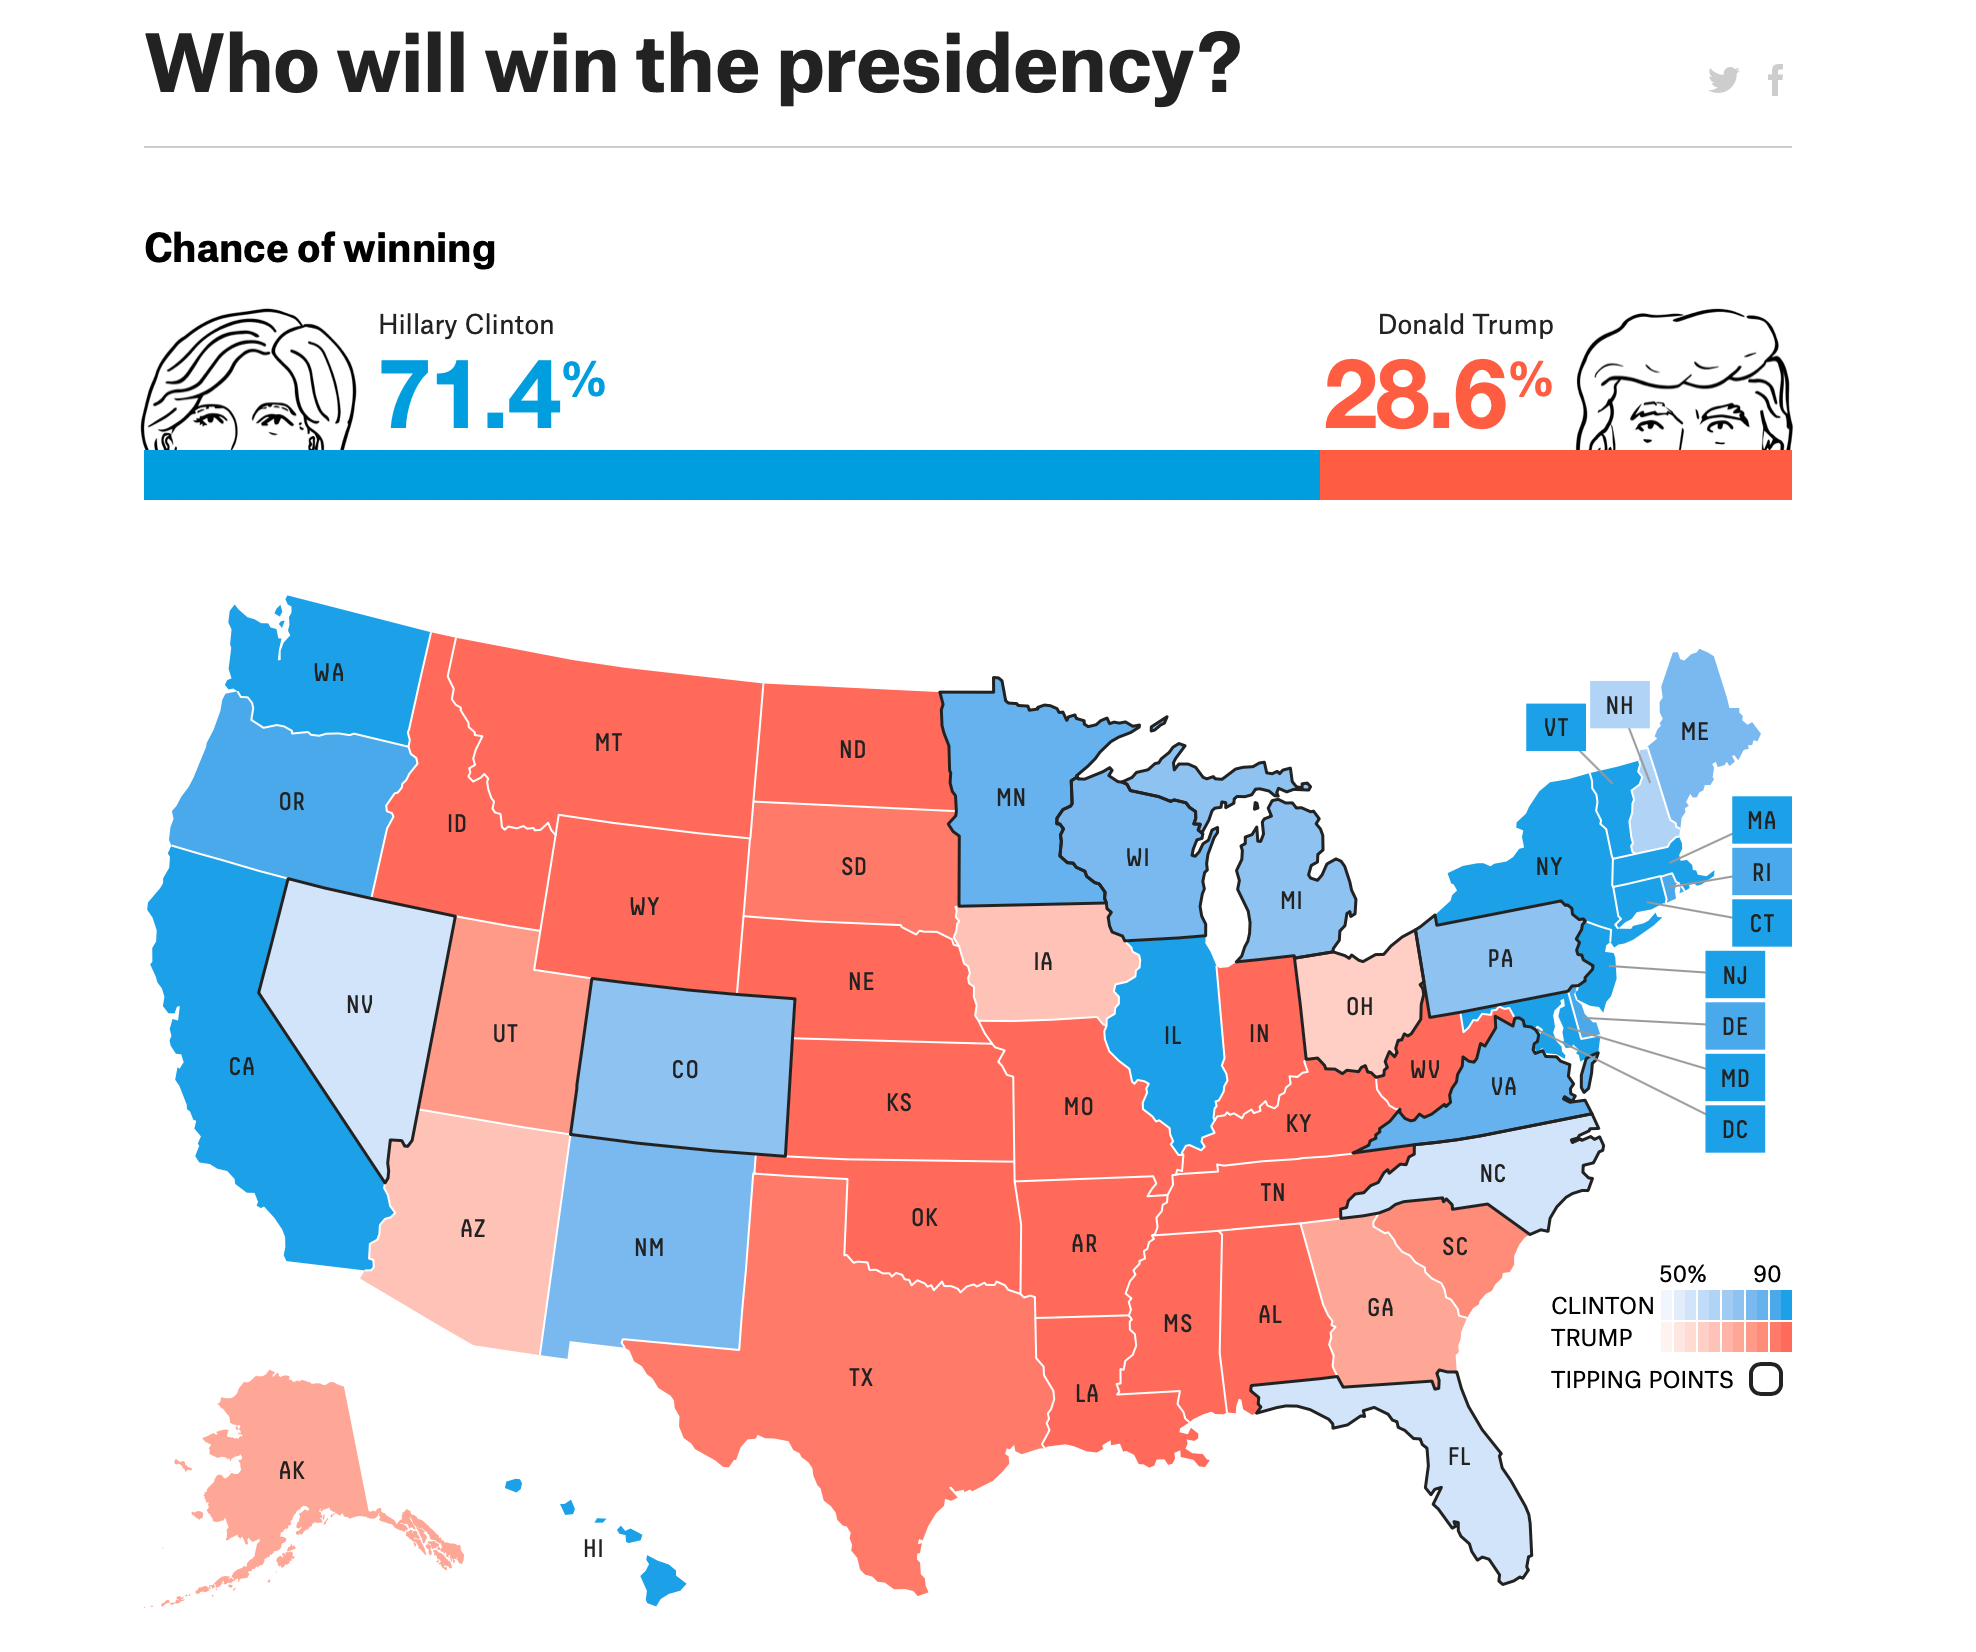
\includegraphics{images/map.png}
\caption{electoral 2016 map}
\end{figure}

\begin{figure}
\centering
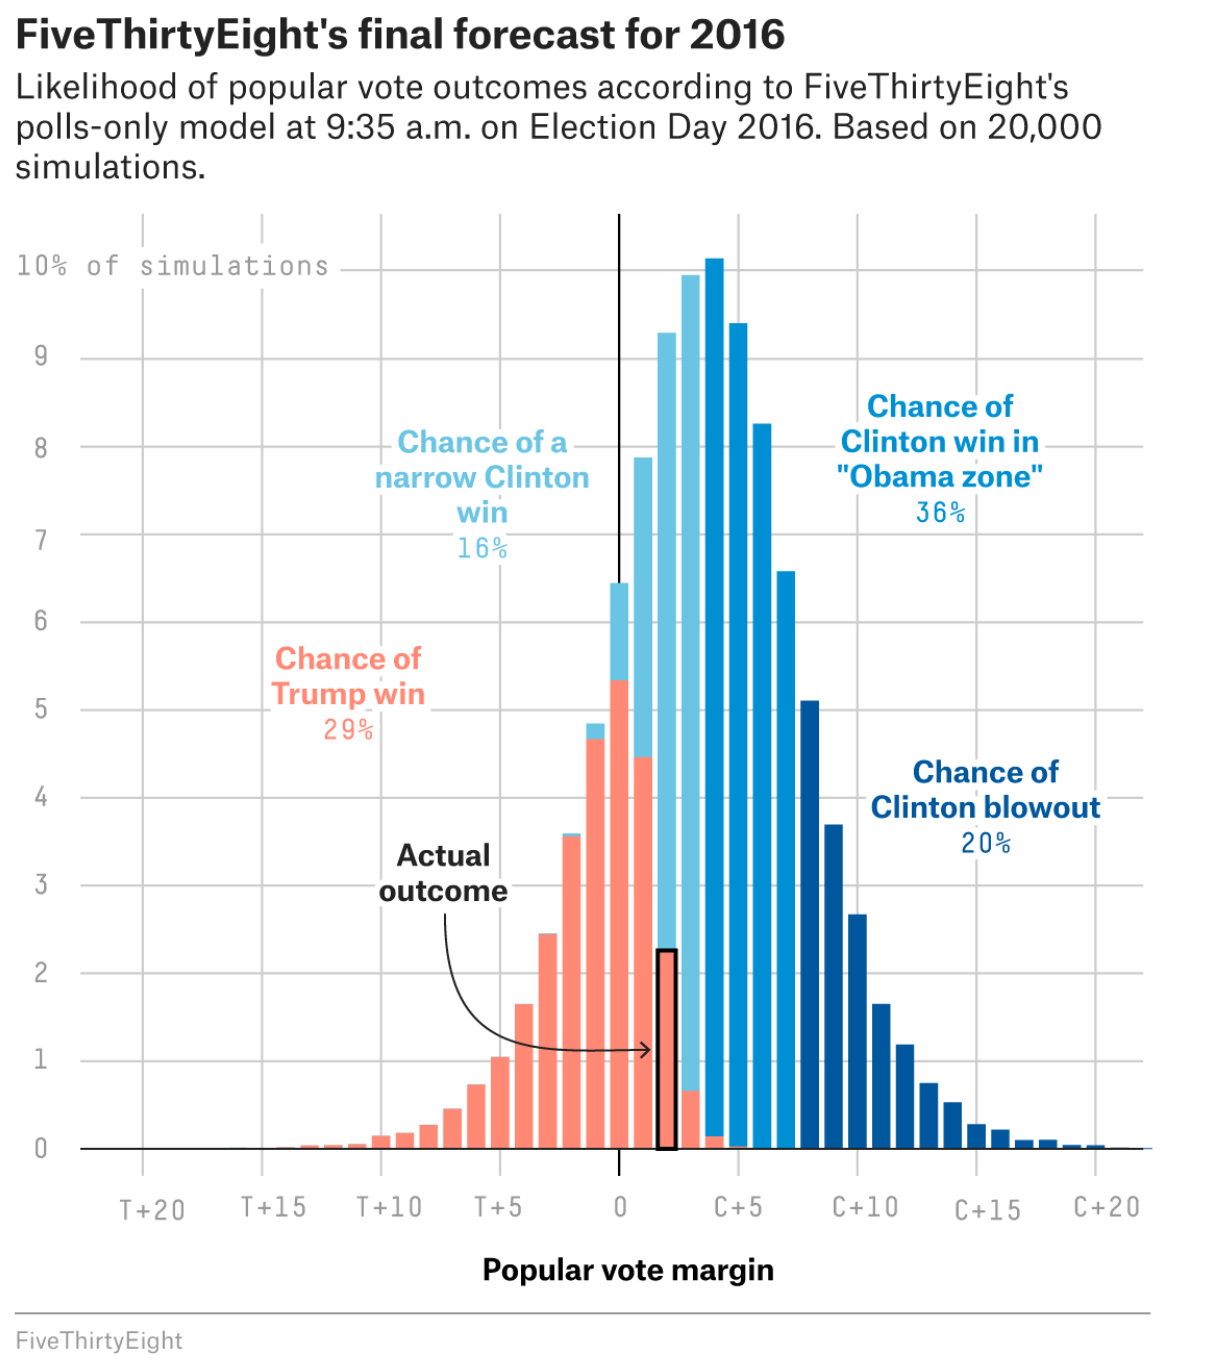
\includegraphics{images/uncertain_dist.png}
\caption{distribution of possible results}
\end{figure}

\hypertarget{use-assumptions-and-document-them}{%
\section{Use Assumptions, and Document Them}\label{use-assumptions-and-document-them}}

(create dummy model regarding time saved through learning democratic data practices)

\hypertarget{dont-get-out-over-your-skis}{%
\section{Don't get out over your skis}\label{dont-get-out-over-your-skis}}

\#\#Practices

Talk about modeling implies math or statistics, when it really doesn't. All a model seeks to do is to simply phenomena in a manner that can be comprehended and used to make decisions in conjunction with subject matter expertise.

\hypertarget{audience-focused}{%
\chapter{Audience-Focused}\label{audience-focused}}

\hypertarget{show-and-tell}{%
\section{Show and Tell}\label{show-and-tell}}

\#\#Vizualizaiton is anything that presents your evidence-- think critically about it!

\hypertarget{applications}{%
\chapter{Applications}\label{applications}}

\hypertarget{tying-it-all-together}{%
\section{Tying it all together}\label{tying-it-all-together}}

\bibliography{book.bib,packages.bib}

\end{document}
